Supomos agora nosso sistema novamente controlado por um banho térmico. Desta vez permitiremos a troca de temperatura e partículas. Definiremos uma energia livre tal que $U(S,V,N) \mapsto \Phi(T,V,\mu)$. Chamaremos esta energia livre de Grão Potencial ou Potencial de Landau. Como sempre, definiremos o potencial como uma transformada de Legendre sob a Energia

\begin{equation}
	\Phi = U - TS - \mu N
\end{equation}

\[
	\Phi(T,V,\mu) = U(S(T,V,\mu), V, N(T,V,\mu)) - TS(T,V,\mu) - \mu N(T,V,\mu)
\]

e é claro, na diferencial

\[
	d\Phi = dU - Tds - SdT - \mu dN - Nd\mu
\]

Onde lembramos que $d\Phi = TdS - PdV + \mu dN$ de forma que

\[
	d\Phi = -SdT - PdV - Nd\mu
\]

Ou seja,

\[
	S = - \left| \frac{\partial \Phi}{\partial T} \right|_{V,N} 
\]
\[
	N = - \left| \frac{\partial \Phi}{\partial \mu} \right|_{T,V} 
\]

Tratamos do seguinte sistema,

\begin{center}
	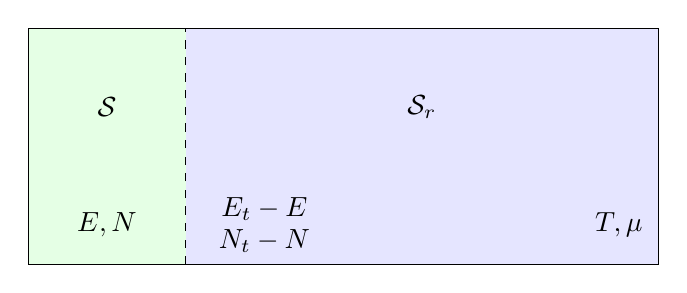
\begin{tikzpicture}
		\fill[blue!10!white] (0,0) rectangle (8,3);
		\fill[green!10!white] (0,0) rectangle (2,3);
		\draw (0,0) rectangle (8,3);
		\draw[dashed] (2,0) -- (2,3);
		\node at (1,2) {$\mathcal{S}$};
		\node at (1,0.5) {$E,N$};
		\node at (5,2) {$\mathcal{S}_r$};
		\node at (7.5,0.5) {$T,\mu$};
		\node at (3,0.7) {$E_t - E$};
		\node at (3,0.3) {$N_t - N$};
	\end{tikzpicture}
\end{center}

Sabemos afirmar que $p_{\sigma} \propto \Omega_R (E_t - E, N_t - N)$, ou seja, cada microestado do nosso sistema é proporcional às formas que o banho pode se arranjar dado $(E,N)$. Ou seja

\begin{align*}
	p_{\sigma} & = \exp{ \lbrace \log{[\Omega_R(E_t - E, N_t - N)]} } \rbrace \\
	& \propto exp{\left\lbrace \frac{1}{k_b} \left[  k_b \log{(\Omega_R(E_T, N_T))} - E \frac{\partial}{\partial E'} (k_b log{\Omega_R(E', N')})\middle|_{N'=N_T}^{E'=E_T} -  N \frac{\partial}{\partial N'} (k_b log{\Omega_R(E', N')})\middle|_{N'=N_T}^{E'=E_T} \right]  \right\rbrace} \\
	& \propto \exp{\left\lbrace  \frac{1}{k_b} \left[  - E \frac{\partial}{\partial E'} (k_b log{\Omega_R(E', N')})\middle|_{N'=N_T}^{E'=E_T} -  N \frac{\partial}{\partial N'} (k_b log{\Omega_R(E', N')})\middle|_{N'=N_T}^{E'=E_T} \right] \right\rbrace}
\end{align*}

Onde retiramos o termo que não depende do nosso sistema de interesse e será constante, agregando ele na proporcionalidade. Agora faremos uso da ideia da entropia como $S = k_b \log{(\Omega_R(E',N'))}$ para escrever a relação acima em termos da temperatura e potencial químico. Usando das derivadas parciais da entropia em $dS = \frac{1}{T} dU + \frac{P}{T} dV - \frac{\mu}{T} dN$,

\begin{align*}
	p_{\sigma} & \propto \exp{\left\lbrace  \frac{1}{k_b} \left[  -E \frac{1}{T} - N \frac{\mu}{T} \right]  \right\rbrace} \\
	& \propto e^{-\beta E + \beta \mu N}
\end{align*}

e

\begin{equation}
	p_\sigma = \frac{1}{\Xi} e^{-\beta E + \beta \mu N}
\end{equation}

Onde 

\begin{equation}
	\Xi = \sum_\sigma e^{-\beta E + \beta \mu N}
\end{equation}

O log da nossa função partição deve resultar em uma expressão de energia livre.

\begin{align*}
	\log{\Xi} & = \log{ \left( \sum_\sigma e^{-\beta E_\sigma + \beta \mu N_\sigma} \right) } \\
	& = \log{ \left( \sum_{E,N}  \Omega(E,N) e^{-\beta E + \beta \mu N} \right) } \\
	& = \log{ \left( \sum_{E,N}  \exp{\left\lbrace \frac{k_b}{k_b} \log{\Omega(E,N)}\right\rbrace}  \exp{\left\lbrace (-\beta E + \beta N \mu) \right\rbrace} \right) } \\
	& = \log{ \left( \sum_{E,N}  \exp{\left\lbrace \frac{T}{k_b T} S - \beta E + \beta N \mu \right\rbrace} \right) } \\
	& = \log{ \left( \sum_{E,N}  e^{ \beta(E - TS - N \mu)} \right) } \\
\end{align*}

Para a aproximação desta expressão vamos considerar que o logaritmo de uma somatória pode ser aproximada por seu termo máximo,

\[
	\approx \log{ e^{ \beta(E^* - TS(E^*,N^*) - N^* \mu)}} = \beta(E^* - TS(E^*,N^*) - N^* \mu)
\]

Ou seja,

\[
\log{\Xi} = \beta(E^* - TS(E^*,N^*) - N^* \mu) = -\beta \Phi
\]

e finalmente,

\begin{equation}
	\Phi = -k_b T \log{\Xi}
\end{equation}